\documentclass[notitlepage, reprint, nofootinbib]{revtex4-1}
\usepackage[utf8]{inputenc}

% Mathematics and symbols:
\usepackage{amsmath, gensymb, amsthm, physics, mhchem}
% Figures:
\usepackage{tikz, graphicx}
\usepackage[caption=false]{subfig}

% Other:
\usepackage{hyperref}

\hypersetup{
    colorlinks=true,
    linkcolor=purple,
    filecolor=magenta,      
    urlcolor=green,
}

\usepackage{algorithm}
\usepackage{algpseudocode}


% Document formatting 
\setlength{\parskip}{1mm}
\setlength{\parindent}{0mm}


%\renewcommand{\thesubsubsection}{\alph{subsubsection})}


\begin{document}
\title{FYS3150 - Project 4}
\author{Frida Larsen}

\begin{abstract}
{\color{red}{The best abstract there ever was.}}
\end{abstract}

\maketitle

\section{Introduction}

\section{Theory: The Ising Model}
As previously mentioned, the Ising model is widely used for simulating phase transitions. Spins in a 2D lattice are represented by arrows pointing up or down. $\uparrow$ indicates a spin value of 1, whilst $\downarrow$ indivates a spin value of -1. \\[2mm]
In the Ising model, assuming no externally applied magnetic field, the energy can be expressed as 
\begin{equation}\label{Ising_energy}E=-J\sum_{<kl>}^Ns_ks_l,\end{equation}
where $N$ is the total number of spins in the system, $J$ is a coupling constant. $s_k$ and $s_l$ are the values of the spins, and can be $\pm1$. The sum is over neighbouring spins, and each pair $k,l$ are counted only once. \\[2mm]
For this project, we will use periodic boundary conditions\footnote{Another option is free ends. The way the boundaries are treated become less significant for larger systems.}. See {\color{red}{figure - see doodle above 'becomes a torus' in notebook!}} for an illustration of the 2x2 case.\\[2mm]
The magnetization of a given configuration is given by
\begin{equation}\label{magnetization}\mathcal{M}_i=\sum_{k=1}^N s_k.\end{equation}


\subsection{Statistical Physics}
Canonical ensemble. Insert distribution.\\[2mm]
The statiscial properties of a system in thermal equilibrium are described by the partition function, 
\begin{equation}\label{partition_function}Z=\sum_{i=1}^M e^{-\beta E_i},\end{equation}
where $M$ is the total number of microstates. $\beta$ is a constant, given by 
\begin{equation}\label{beta}\beta=\frac{1}{k_BT}.\end{equation}
The partition function can be used to deduct a number of other interesting properties of the system. The mean energy and the mean of energy squared are given by 
\begin{equation}\label{mean_energy}\langle E\rangle =\frac{1}{Z}\sum_{i=1}^ME_ie^{-\beta E_i}\end{equation}
and
\begin{equation}\label{mean_energy_2}\langle E^2\rangle = \frac{1}{Z}\sum_{i=1}^M E_i^2 e^{-\beta E_i}.\end{equation}
The mean magnetization is 
\begin{equation}\label{mean_mag}\langle \mathcal{M}\rangle =\frac{1}{Z}\sum_{i=1}^M\mathcal{M}_i e^{\beta E_i},\end{equation}
where $\mathcal{M}_i$ is given by equation \ref{magnetization}. The mean of the magnetization squared is given by 
\begin{equation}\label{mean_mag2}\langle \mathcal{M}^2\rangle =\frac{1}{Z}\sum_{i=1}^M\mathcal{M}_i^2 e^{\beta E_i},\end{equation}
The specific heat of a system is the amount of heat that must be added (as heat) to the system in order to increase the temperature of one unit by one unit. If the substance being heated is allowed to expand as it is being heated, the specific heat is said to be at constant pressure. If the substance is heated in an enclosed space, however, the specific hest is said to be at constant volume. In the latter case, the specific heat is given by 
\begin{equation}\label{specific_heat}C_V = \frac{1}{k_BT^2}(\langle E^2\rangle - \langle E\rangle^2).\end{equation}
The susceptibility of a substance is a measure of how much the material will become magnetized if a magnetic field is applied and is given by 
\begin{equation}\label{susceptibility}\chi = \beta (\langle \mathcal{M}^2\rangle -\langle \mathcal{M}\rangle^2).\end{equation}

\subsection{The 2x2 case}
Consider a 2x2 lattice of spins. There are $2^4=16$ possible configurations. The expression for the energy from equation \ref{Ising_energy} can be written out as 
\begin{equation}\label{Ising_energy_2x2}E_i = s_1s_2+s_2s_1+s_3s_4+s_4s_3+s_3s_1+s_1s_3+s_2s_4+s_4s_2,\end{equation}
where the spins are labeled as in {\color{red}{figure}}. Table \ref{2x2_table} lists the degeneracy, energy and magnetization of each possible configuration. 
\begin{table}[]
\centering
\begin{tabular}{|l|l|l|l|}
\hline
Number of $\uparrow$ & Degeneracy & Energy ($E_i$) & Magnetization ($\mathcal{M}_i$) \\ \hline
4 & 1 & -8J & 4 \\ \hline
3 & 4 & 0 & 2 \\ \hline
2 & 4 & 0 & 0 \\ \hline
2 & 2 & 8J & 0 \\ \hline
1 & 4 & 0 & -2 \\ \hline
0 & 1 & -8J & -4 \\ \hline
\end{tabular}
\caption{Degeneracy, energy and magnetization of all configurations of spins in a 2x2 lattice.}
\label{2x2_table}
\end{table}
The partition function is given by 
\begin{align*}
	Z_{2x2}&=e^{-\beta(-8J)}+4e^0+4e^0+2e^{-\beta(8J)}+4e^0+e^{-\beta(-8J)}\\
	&= 2e^{8\beta J}+2e^{-8\beta J}+12.
\end{align*}
The mean energy and the mean squared energy is given by 
\begin{align*}
	\langle E\rangle&=\frac{1}{2e^{8\beta J}+2e^{-8\beta J}+12}\Big(-8Je^{8\beta J}+16Je^{-8\beta J}-8Je^{8\beta J}\Big)\\
	&=\frac{8Je^{-8\beta J} - 8Je^{8\beta J}}{e^{8\beta J}+e^{-8\beta J}+6}
\end{align*}
and 
\begin{align*}
	\langle E^2\rangle &=\frac{1}{2e^{8\beta J}+2e^{-8\beta J}+12}\Big((-8J)^2e^{8\beta J}+2(8J)^2e^{-8\beta J}+(-8J)^2e^{8\beta J}\Big)\\
	&=\frac{64J^2e^{-8\beta J} + 64J^2e^{8\beta J}}{e^{8\beta J}+e^{-8\beta J}+6}.
\end{align*}
Thus the specific heat capacity becomes 
\begin{equation*} C_V=\frac{1}{k_BT^2}\Big(\frac{64J^2e^{-8\beta J} + 64J^2e^{8\beta J}}{e^{8\beta J}+e^{-8\beta J}+6} - \Big[\frac{8Je^{-8\beta J} - 8Je^{8\beta J}}{e^{8\beta J}+e^{-8\beta J}+6}\Big]^2\Big).\end{equation*}
For the mean magnetization and the mean square magnetization we get 
\begin{align*}
	\langle M\rangle &= \frac{1}{2e^{8\beta J}+2e^{-8\beta J}+12}\Big(4e^{8\beta J}+2e^0-2e^0-4e^{8\beta J}\Big)\\
	&=0
\end{align*}
and
\begin{align*}
	\langle M^2 \rangle &=\frac{1}{2e^{8\beta J}+2e^{-8\beta J}+12}\Big(16e^{-8\beta J}+4e^0+4e^0+16e^{8\beta J}\Big)\\
	&= \frac{8e^{-8\beta J}+8e^{8\beta J}+4}{e^{8\beta J}+e^{-8\beta J}+6}.
\end{align*}
Thus the susceptibility becomes 
\begin{align*}
	\chi &= \frac{1}{k_BT}\Big(\frac{8e^{-8\beta J}+8e^{8\beta J}+4}{e^{8\beta J}+e^{-8\beta J}+6} - 0\Big)\\
	&=\frac{1}{k_BT} \frac{8e^{-8\beta J}+8e^{8\beta J}+4}{e^{8\beta J}+e^{-8\beta J}+6}.
\end{align*}
{\color{red}{Figure out why dividing by 4 is necessary for numerical chi.....}}

\subsection{Phase transitions}

\section{Method}
\subsection{The Metropolis algorithm}

\section{Results}
The numerical calculation of the mean energy, mean absolute magnetization, specific heat and susceptibility are compared to the analytic values in figures \ref{fig1}, \ref{fig2}, \ref{fig3} and \ref{fig4}. We see a significant leap in accuracy around $10^4$ for all four thermodynamic variables. 
\begin{figure}
	\centering
	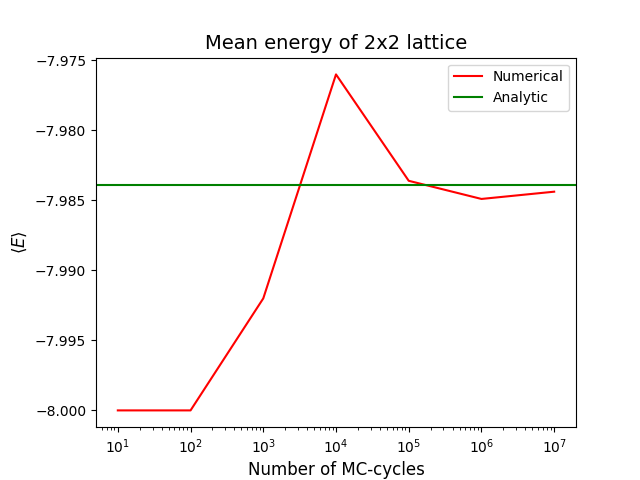
\includegraphics[width=0.45\textwidth]{../Figures/E_mean_4b.png}
	\caption{The mean energy of a 2x2 lattice computed numerically and analytically}
	\label{fig1}
\end{figure}

\begin{figure}
	\centering
	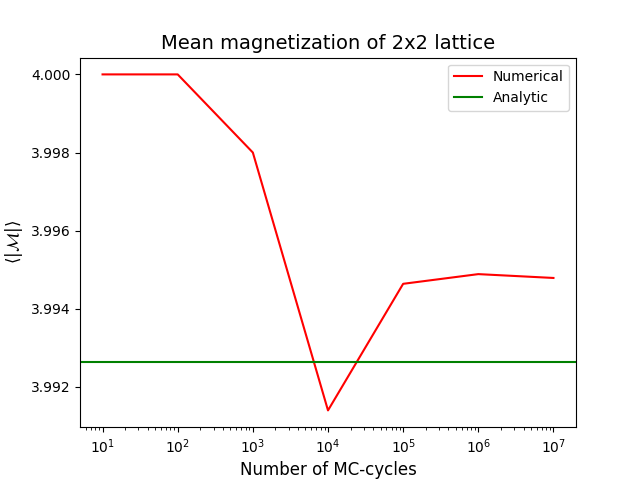
\includegraphics[width=0.45\textwidth]{../Figures/M_mean_4b.png}
	\caption{The mean absolute magnetization of a 2x2 lattice computed numerically and analytically}
	\label{fig2}
\end{figure}

\begin{figure}
	\centering
	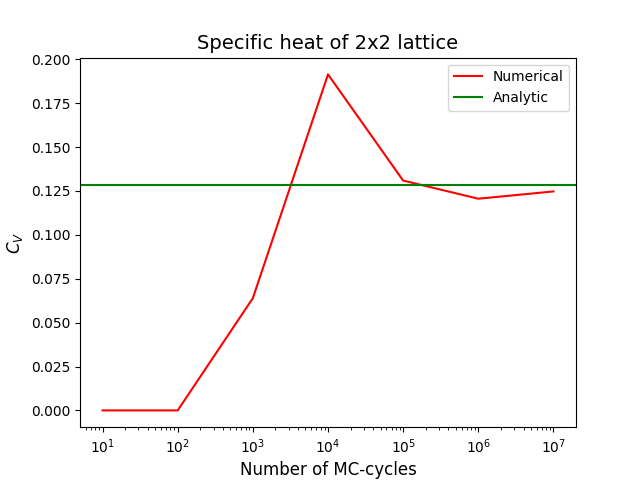
\includegraphics[width=0.45\textwidth]{../Figures/C_V_4b.png}
	\caption{The specific heat of a 2x2 lattice computed numerically and analytically}
	\label{fig3}
\end{figure}

\begin{figure}
	\centering
	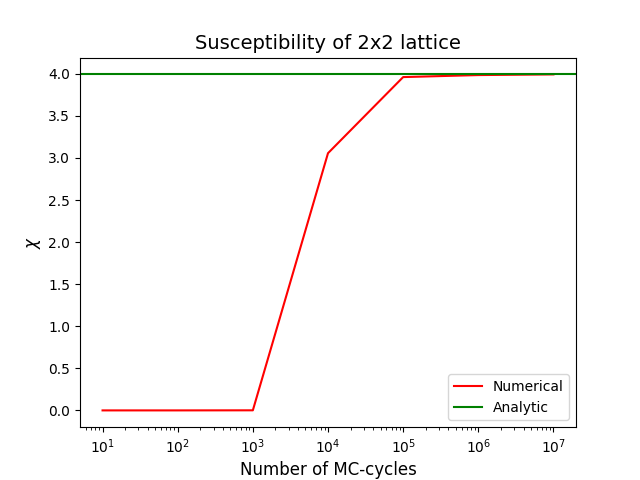
\includegraphics[width=0.45\textwidth]{../Figures/chi_4b.png}
	\caption{The susceptibility of a 2x2 lattice computed numerically and analytically}
	\label{fig4}
\end{figure}

\section{Discussion}

\section{Conclusion}


\onecolumngrid
\bibliographystyle{unsrtnat}
\bibliography{fridala_project_4Notes.bib}










\end{document}